% Meridional sketch of the annulus coordinate (m, spf).
%
% Two blade rows drawn in the meridional plane: horizontal hub and casing
% lines, each row a pair of vertical leading- and trailing-edge lines with a
% diagonal cross joining the four corners. The normalised meridional
% coordinate m runs 0 at the inlet, odd integers at leading edges, even
% integers at trailing edges; the span fraction spf runs 0 at the hub to 1 at
% the casing.
%
% Build:  pdflatex annulus_coordinate.tex
%         dvisvgm --pdf --no-fonts --output=../_static/annulus_coordinate.svg annulus_coordinate.pdf
% (or use  make -C doc figures)

\documentclass[border=4pt]{standalone}
\usepackage{tikz}
\usepackage{newtxtext,newtxmath}
\usetikzlibrary{arrows.meta}

\def\spanmax{1.5}  % hub-to-casing height in figure units

\begin{document}
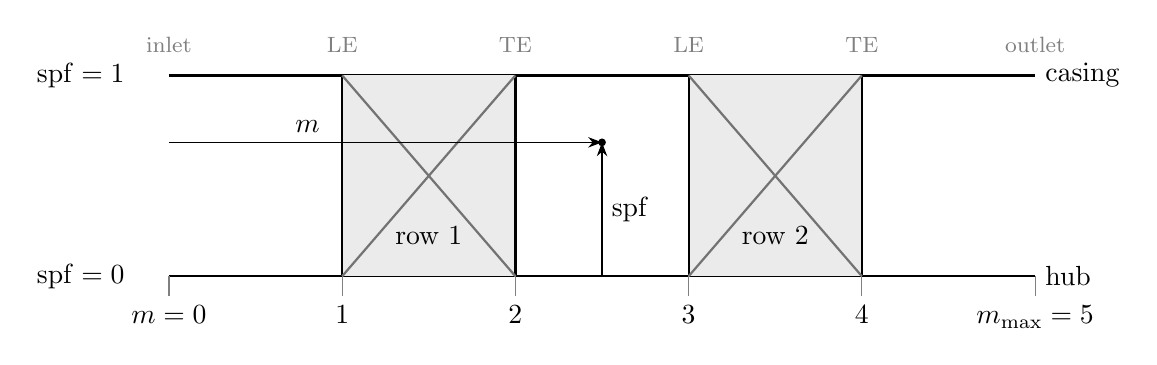
\begin{tikzpicture}[
    x=2.2cm, y=1.7cm,
    line/.style={thick},
    row/.style={fill=black!8},
    edge/.style={thick},
    cross/.style={thick, black!55},
    dim/.style={-{Stealth[length=5pt]}, gray},
    tick/.style={gray},
  ]

  % --- hub and casing lines -------------------------------------------------
  \draw[line] (0,0) -- (5,0) node[right] {hub};
  \draw[line] (0,\spanmax) -- (5,\spanmax) node[right] {casing};

  % --- blade rows: LE/TE verticals + diagonal cross -----------------------
  \foreach \le/\lab in {1/1, 3/2} {
    \pgfmathsetmacro\te{\le+1}
    \fill[row] (\le,0) rectangle (\te,\spanmax);
    \draw[edge] (\le,0) -- (\le,\spanmax);
    \draw[edge] (\te,0) -- (\te,\spanmax);
    \draw[cross] (\le,0) -- (\te,\spanmax);
    \draw[cross] (\le,\spanmax) -- (\te,0);
    \node at ({(\le+\te)/2},0.3) {row \lab};
  }

  % --- meridional coordinate ticks and labels ----------------------------
  \foreach \m/\lab in {0/{$m=0$}, 1/1, 2/2, 3/3, 4/4, 5/{$m_\mathrm{max}=5$}} {
    \draw[tick] (\m,0) -- (\m,-0.15);
    \node[below] at (\m,-0.15) {\lab};
  }
  % roles of the integer stations
  \foreach \m/\role in {0/inlet, 1/LE, 2/TE, 3/LE, 4/TE, 5/outlet} {
    \node[gray, above, font=\footnotesize] at (\m,{\spanmax+0.1}) {\role};
  }

  % --- span fraction labels ---------------------------------------------
  \node[left] at (-0.2,0)        {$\mathrm{spf}=0$};
  \node[left] at (-0.2,\spanmax) {$\mathrm{spf}=1$};

  % --- an example point, addressed by (m, spf) -------------------------
  \fill[black] (2.5,1.0) circle (1.4pt);
  \draw[dim, black] (0,1.0) -- (2.5,1.0) node[pos=0.32, above] {$m$};
  \draw[dim, black] (2.5,0) -- (2.5,1.0) node[midway, right] {$\mathrm{spf}$};

\end{tikzpicture}
\end{document}
